%!TEX program = xelatex
\documentclass{xmu}

%%%%%%%%%%%%%%%%%%%%%%%%%%%%%%%%%%%%%%%%%%%%%%%%%%%%%%%%%%%%%%%
%%%%%%%%  XMU Undergraduates English Thesis Template   %%%%%%%%
%%%%%%%%             Made by: F5Soft                   %%%%%%%%
%%%%%%%%             Adpated by: Haoran Yu            %%%%%%%%
%%%%%%%%  https://github.com/ha0ranyu/xmu-template-en  %%%%%%%%
%%%%%%%%%%%%%%%%%%%%%%%%%%%%%%%%%%%%%%%%%%%%%%%%%%%%%%%%%%%%%%%

% 如果需要使用 bib 文件导入参考文献,则取消注释下一行
\bibliography{references.bib}

\begin{document}

% 电子版 / 打印版(取消注释下一行即为打印版)
\print
% 取消注释后,将在某些偶数页产生空白页,使得下一部分的内容从奇数页开始

% 取消注释后,仅使用数字作为章的编号
% 注:必须取消注释,否则使用 \ref{ch:...} 时将出现汉字数字!
\arabicchapter

% 毕业设计 / 毕业论文(取消注释下一行即为毕业设计)
% \design

% 主修 / 辅修(取消注释下一行即为辅修)
% \minor

% 标题
\title{厦门大学本科毕业论文LaTeX模版}
{A LaTeX Template of Xiamen University Undergraduate Thesis}

% 姓名
\author{F5Soft.site}

% 学号
\idn{22920182200000}

% 学院
\college{信息学院}

% 专业
\subject{计算机科学与技术}

% 年级
\grade{2018级}

% 校内指导教师
\teacher{F5Soft\; 副教授}

% 校外指导教师(注释则不显示)
\otherteacher{F5Soft\; 教授}

% 完成时间
\pubdate{二〇二二年四月三十日}

% 关键词
\keywords{本科毕业论文;LaTeX;厦门大学}
{Undergraduate Thesis; LaTeX; Xiamen University}

% 生成封面、承诺书
\maketitle

% 如果想要将致谢放在最前,可将最后的致谢移动至此
%%%%%%%% 致谢(默认在最后) %%%%%%%%

\begin{acknowledgement}
    Although the ``Xiamen University Undergraduate Thesis (Design) Guidelines'' (《厦门大学本科毕业论文(设计)规范》) stipulate that the acknowledgments should be placed in the preliminary sections, in most cases, acknowledgments are typically placed at the end of the thesis.
    \par
    The ``Guidelines'' also emphasize that the acknowledgments should briefly express gratitude to those who directly assisted in the research and writing process of the thesis (such as advisors, instructors, and other individuals).
    Therefore, if this template has been helpful for your thesis, you might consider mentioning it in the acknowledgments.
\end{acknowledgement}

%%%%%%%% 摘要 %%%%%%%%

% 中文摘要
\begin{abstract}
    本模版基于厦门大学图书馆i学堂LaTeX讲座中提供的硕博毕业论文模版 \parencite{xmuischool} 改编而来,并根据《厦门大学本科毕业论文(设计)规范》\parencite{xmuthesis} 进行了大幅度的格式调整。本模版提供高清封面、诚信承诺书、中英文摘要环境、中英文目录自动生成、附录环境、参考文献环境、致谢环境等。本模版还自带了Windows中的中易宋体、中易黑体、中易楷体、中易仿宋字体,以兼容缺少这些字体的Linux和macOS系统。
\end{abstract}

% 英文摘要
\begin{enabstract}
    This template is adapted from the master and doctoral dissertation template provided in the LaTeX lecture of Xiamen University Library i-School \parencite{xmuischool}, and has been greatly adjusted according to the \textit{Xiamen University Undergraduate Thesis (Design) Specifications} \parencite{xmuthesis}. This template provides high-definition cover, letter of declaration, Chinese and English abstract environment, automatic generation of table of contents in Chinese and English, appendix environment, reference environment, acknowledgements environment, etc. This template also comes with SimSun, SimHei, SimKai, and SimFang fonts in Windows to be compatible with Linux and macOS systems which lack these fonts.
\end{enabstract}

% 生成中英文目录
\tableofcontents

%%%%%%%% 正文 %%%%%%%%

\xmuchapter{使用说明}{Introduction} \label{ch:Introduction}
\xmusection{环境配置}{Environment Setup} \label{sec:Environment Setup}
First, you need to set up the LaTeX environment. It is recommended to use TeX Live + VSCode. TeX Live can be downloaded from {https://www.tug.org/texlive/}, and after installing VSCode, you will need to search for and install the LaTeX Workshop extension.
\xmusection{编译}{Compiling}
Once the environment is set up, you can download the code for this template from GitHub \parencite{template}. After downloading, try opening the example.tex file and click the green run button in the top right corner to compile. On macOS systems, the compilation will usually fail due to pdflatex not being able to find the corresponding Chinese fonts. To resolve this, go to the LaTeX Workshop panel on the left, select ``Recipe'' as latexmk (xelatex), and click run to compile successfully.
\xmusection{使用模版}{Use Templates}
This template encapsulates a large number of formatting settings based on the ``Xiamen University Undergraduate Thesis (Design) Guidelines'' \parencite{xmuthesis}, so that users do not need to worry about various formatting commands. All you need to do is set the chapter titles and fill in the abstract, appendix, references, acknowledgments, and other sections.
\xmusubsection{示例论文}{Example Paper}
The example.tex file contains detailed comments and usage examples, which you can directly modify based on the provided example. All illustrations in the thesis should be placed in the ``figures'' folder and included according to their file names.
\xmusubsection{自定义模版}{Customization}
The xmu.cls file is the template file. If you have a perfectionist tendency towards typesetting and wish to fine-tune the template details like I did, you can modify the xmu.cls template file yourself. The template file also includes many comments to assist you in making changes. If you are satisfied with the modifications, you can contribute by submitting a pull request on GitHub \parencite{template}. You can also open an issue to suggest features you would like to add.
\par
Modifying the template requires a certain level of LaTeX knowledge. You can refer to the ``LaTeX 2e Complete Learning Manual'' (《LaTeX 2e完全学习手册》) \parencite{latex2e} and ``Simple and Straightforward LaTeX'' (《简单粗暴LaTeX》) \parencite{easylatex} for guidance on making changes.
\xmuchapter{使用示例}{Examples}
\xmusection{二级标题}{Section (English Ver.)}
A first-level heading (chapter) will always start on a new page.
\xmusubsection{三级标题}{Subsection (English Ver.)}
Use the xmuchapter, xmusection, and xmusubsection commands to specify the first-level (chapter), second-level (section), and third-level (subsection) headings. Due to the requirements for a bilingual table of contents, each of these three commands takes two parameters: the first parameter is the title in Chinese, and the second parameter is the title in English.
\subsubsection{Subsubsection (English Ver.)}
If a fourth-level heading is required, it will not appear in the table of contents.
\xmusection{图表}{Figures and Tables}
\xmusubsection{插图}{Figures}
Images are numbered according to the chapter number and the image number (e.g., chapter number-image number). The caption for the image can be set using the caption command, and the image number can be referenced using the label and ref commands. The Xiamen University logo is shown in the figure below \ref{xmulogo}.
\begin{figure}[!htb]
    \centering
    \includegraphics[width=12em]{xmu-logo-icon.jpg}\\
    \caption{Xiamen University logo}\label{xmulogo}
\end{figure}
According to the ``Xiamen University Undergraduate Thesis (Design) Guidelines'' \parencite{xmuthesis}, the title and figure number of the image should be placed at the center below the image. Below is an example showing two images side by side:
\begin{figure}[!htb]
    \begin{minipage}{0.5\linewidth}
        \centering
        \includegraphics[height=5em]{xmu-logo-icon.jpg}
        \caption{Xiamen University logo}\label{xmu1}
    \end{minipage}
    \begin{minipage}{0.5\linewidth}
        \centering
        \includegraphics[height=5em]{xmu-logo-text.jpg}
        \caption{Xiamen University text}\label{xmu2}
    \end{minipage}
\end{figure}
\xmusubsection{表格}{Tables}
For tables, the numbering follows the format chapter number-table number. Similarly, the table caption can be set using the caption command, and the table number can be referenced using the label and ref commands. The table \ref{database} below shows an example of a database table design.
\begin{table}[!htb]
    \centering
    \caption{Basic Information Table}
    \label{database}
    \begin{tabular}{|l|l|l|l|l|}
        \hline
        \bf\songti Field Name & \bf\songti Field Type & \bf\songti Length & \bf\songti Field Description & \bf\songti Notes \\ \hline
        Account Number    & Number          & 30            &                               & Primary Key   \\ \hline
        Password          & Number          & 30            & Encrypted                     &               \\ \hline
        Name              & Varchar         & 50            &                               &               \\ \hline
        Email Address     & Varchar         & 50            & Required for VIP customers    &               \\ \hline
    \end{tabular}
\end{table}
According to the ``Xiamen University Undergraduate Thesis (Design) Guidelines'' \parencite{xmuthesis}, the title and table number should be placed at the center above the table. The font for the table content should be 5-point Songti, and the font for the table header should be 5-point bold Songti.
\xmusection{画图}{Plotting}
The tikzpicture environment can be used to draw functions, line charts, scatter plots, etc., as shown in Figure \ref{plot}.
\begin{figure}[!htbp]
    \centering
    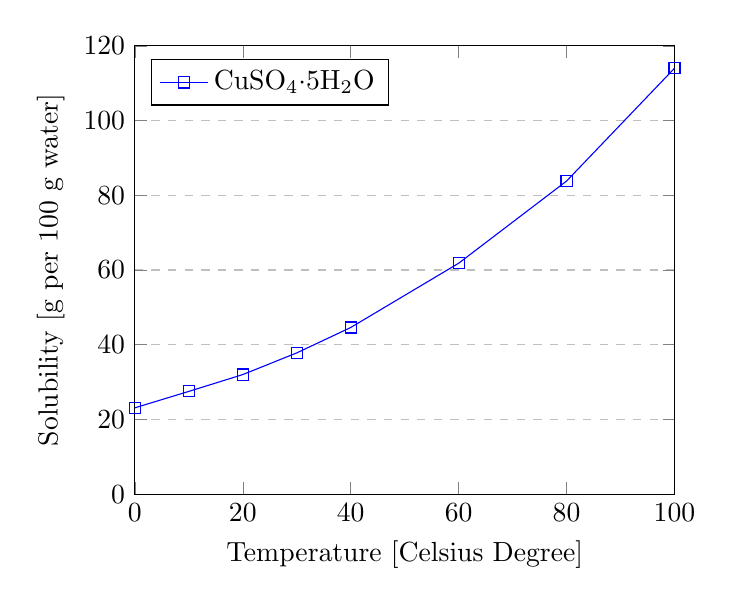
\begin{tikzpicture}
        \begin{axis}[
                xlabel={Temperature [Celsius Degree]},
                ylabel={Solubility [g per 100 g water]},
                xmin=0, xmax=100,
                ymin=0, ymax=120,
                xtick={0,20,40,60,80,100},
                ytick={0,20,40,60,80,100,120},
                legend pos=north west,
                ymajorgrids=true,
                grid style=dashed,
            ]

            \addplot[
                color=blue,
                mark=square,
            ]
            coordinates {
                    (0,23.1)(10,27.5)(20,32)(30,37.8)(40,44.6)(60,61.8)(80,83.8)(100,114)
                };
            \legend{CuSO\(_4\cdot\)5H\(_2\)O}

        \end{axis}
    \end{tikzpicture}
    \caption{Temperature dependence of CuSO\(_4\cdot\)5H\(_2\)O solubility}\label{plot}
\end{figure}
\xmusection{公式}{Formulas}
Formulas can be divided into inline formulas $a^2+b^2=c^2$ and display formulas:
$$
    \int_a^b\int_a^x\int_x^{x^2}(3y+7)z\;\mathrm{d}z\,\mathrm{d}y\,\mathrm{d}x
$$
$$
    |-0.75|^{2}+(5.5-4.2)^2+\sqrt[4.2]{3}+\log_{3.3}{4.7}+\cos1.24\,\sin1.7\approx5.17
$$
If you need to assign a formula number, you can also use the label and ref commands for referencing. The correct result of Equation \ref{eq1} should be $\frac{\sqrt{3}}{6}$。
\begin{equation}\label{eq1}
    \lim_{x\to0}\frac{\displaystyle{\int_{\sin x}^x\sqrt{3+t^2}\,\mathrm{d}t}}{x(e^{x^2}-1)}
\end{equation}
Equation \ref{eq2} provides an example of a matrix. Note that it is better to use boldsymbol rather than bm for bold letters.
\begin{equation}\label{eq2}
    \boldsymbol{Ax} = \boldsymbol{b},\quad\boldsymbol{A} = \left(\begin{array}{ccc}
            a_{11} & a_{12} & a_{13} \\
            a_{21} & a_{22} & a_{23} \\
            a_{31} & a_{32} & a_{33} \\
        \end{array}\right),\quad \boldsymbol{b}=\left(\begin{array}{c}
            b_1 \\ b_2 \\ b_3\end{array}\right)
\end{equation}
Equation \ref{eq3} provides an example of a determinant:
\begin{equation}\label{eq3}
    \left|\begin{array}{cc}
        1 & 2 \\
        3 & 4 \\
    \end{array}\right|=1\times4-2\times3=-2
\end{equation}
Equation \ref{eq4} provides an example of a system of equations:
\begin{equation}\label{eq4}
    \begin{cases}
        mgh=mv_1^2                         \\
        \dfrac12mv_2^2-\dfrac12mv_1^2=F_fs \\
        F_f=\mu mg                         \\
    \end{cases} \Rightarrow s,v_1,F_f
\end{equation}

\xmusection{算法}{Algorithms}
If you only need to display code, you may consider using the verbatim environment\footnote{For more advanced code display, you can consider using the lstlisting environment from the listings package, which supports syntax highlighting, line breaks, line numbering, custom colors, custom fonts, and more.}.
Here is a footnote. You can insert footnotes using the footnote command\footnote{Footnote example.}.
\begin{verbatim}
#include <unistd.h>
int main()
{
    write(STDOUT_FILENO, "Hello, world!\n", 14);
    return 0;
}
\end{verbatim}
If you only need to display an algorithm without showing the actual code, you can use the algorithm environment, as shown in Algorithm \ref{alg1}:
\begin{algorithm}[!htb]
    \KwData{sum, $i$: integer}
    \Begin{
        \For{$i\leftarrow0$ \KwTo $100$ \do}{
            sum $\leftarrow$ sum + $i$\;
            \If{\rm sum $>4000$}{
                \bf break\;
            }
        }
        \bf print \rm$i$\;
    }
    \caption{Loop-based summation algorithm}\label{alg1}
\end{algorithm}

%%%%%%%% 参考文献 %%%%%%%%

\begin{reference}
    % bib 文件可以通过百度学术、Google Scholar 的引用界面自动生成
    % 已自动按照 GB/T 7714-2005 设置参考文献的引用格式
    \printbibliography[title=References]
\end{reference}

%%%%%%%% 附录 %%%%%%%%

\begin{appendix}
    \xmusection{附表}{Tables}
    Here are some contents for the appendix, such as tables or other explanations, like Appendix Table \ref{atable}.
    \begin{table}[!htb]
        \centering
        \caption{Appendix Table Example}
        \label{atable}
        \begin{tabular}{llr}
            \hline
            \multicolumn{2}{c}{Item} &                          \\ \cline{1-2}
            Animal                   & Description & Price (\$) \\ \hline
            Gnat                     & per gram    & 13.65      \\
                                     & each        & 0.01       \\
            Gnu                      & stuffed     & 92.50      \\
            Emu                      & stuffed     & 33.33      \\
            Armadillo                & frozen      & 8.99       \\ \hline
        \end{tabular}
    \end{table}
    The numbering in the appendix begins with the letter ``A.'' For example, Equation \ref{eq5}.
    \begin{equation}\label{eq5}
        \sin \left(2x+\frac\pi2\right)=\frac 12
    \end{equation}
    \xmusection{厦门大学本科毕业论文(设计)规范摘要}{Abstract of Xiamen University Undergraduate Dissertation (Design) Specification}
    主修专业毕业论文(设计)封面使用 160g 白色双胶纸,辅修封面为 160g 浅黄色皮纹纸。内页均为 A4 规格 80g 双胶纸。\par
    章的标题占2行,标题以外的文字为1.5倍行距。\par
    上边距和左边距应留 25mm 以上间隙,下边距和右边距应分别留 20mm 以上间隙。\par
    每页须加“页眉”和“页码”。奇数页页眉内容为当前章名,如“第一章 绪论”。偶数页页眉内容为论文题目。学位论文的页码,正文、参考文献、附录部分用阿拉伯数字连续编码并居中,前置部分用罗马数字单独连续编码居中(封面除外)。\par
    封面中文标题:二号黑体\par
    封面英文标题:三号 Times New Roman 加粗\par
    中文摘要标题:小三号黑体\par
    中文关键词标题:小四号黑体\par
    中文摘要、关键词内容:小四号宋体\par
    英文摘要标题:小三号 Times New Roman 加粗\par
    英文关键词标题:小四号 Times New Roman 加粗\par
    英文摘要、关键词内容:小四号 Times New Roman\par
    中文目录标题:小三号黑体\par
    中文目录中章的标题:四号黑体\par
    中文目录中节的标题:小四号黑体\par
    中文目录中三级标题:小四号宋体\par
    英文目录标题:小三号 Times New Roman 加粗\par
    英文目录中章的标题:四号 Times New Roman 加粗\par
    英文目录中节的标题:小四号 Times New Roman 加粗\par
    英文目录中三级标题:小四号 Times New Roman\par
    章的标题:小三号黑体\par
    节的标题:四号黑体\par
    三级标题:小四号黑体\par
    正文:小四号宋体\par
    页眉:小五号宋体\par
    页码:小五号 Times New Roman\par
    注释内容:小五号宋体\par
    表格、图的标题、单位、表头:五号宋体加粗\par
    表格内容:五号宋体\par
    表格、图的资料来源:小五号宋体\par
    参考文献标题:小三号黑体\par
    中文参考文献表:五号宋体\par
    英文参考文献表:五号 Times New Roman\par
    附录标题:小三号黑体\par
    致谢标题:小三号黑体\par
    致谢内容:小四号宋体\par
    对于中英文混杂的内容,{\bf\songti 中文的字体若是用宋体,英文的字体则采用Times New Roman};{\sf 中文的字体若是黑体,英文的字体则采用Arial}。\footnote{
        因此,本模版提供了如下的几种字体设置。rm:罗马字族,中文宋体,英文Times。sf:等线字族,中文黑体,英文Arial。bf:粗体序列,中文黑体,英文Times加粗。it:斜体序列,中文楷体,英文Times斜体。如果需要使用难看的宋体加粗,则需要通过 \textbackslash bf\textbackslash songti实现。当然,也可以使用 songti、heiti、kaishu 手动指定中文字体,此时英文字体均默认为Times。
    }

    The cover of the thesis (design) for the major should use 160g white double offset paper, while the cover for the minor should use 160g light yellow leather-textured paper. The inner pages should be A4 size with 80g double offset paper.

    The title of each chapter occupies 2 lines, and the line spacing for text other than the title is 1.5 times the normal line spacing.

    The top and left margins should be at least 25mm, and the bottom and right margins should be at least 20mm.

    Each page should include a ``header'' and ``page number''. The header on odd-numbered pages should contain the current chapter title, such as ``Chapter 1 Introduction'', while the header on even-numbered pages should contain the thesis title. The page numbers for the thesis, including the main text, references, and appendices, should be consecutively numbered with Arabic numerals, centered. The preliminary sections should use Roman numerals for page numbers, also centered (excluding the cover page).

    Cover page Chinese title: size 2, boldface black font

    Cover page English title: size 3, bold Times New Roman

    Chinese abstract title: size 3, boldface black font

    Chinese keywords title: size 4, boldface black font

    Chinese abstract and keywords content: size 4, Songti font

    English abstract title: size 3, bold Times New Roman

    English keywords title: size 4, bold Times New Roman

    English abstract and keywords content: size 4, Times New Roman

    Chinese table of contents title: size 3, boldface black font

    Chapter titles in the Chinese table of contents: size 4, boldface black font

    Section titles in the Chinese table of contents: size 4, boldface black font

    Subsection titles in the Chinese table of contents: size 4, Songti font

    English table of contents title: size 3, bold Times New Roman

    Chapter titles in the English table of contents: size 4, bold Times New Roman

    Section titles in the English table of contents: size 4, bold Times New Roman

    Subsection titles in the English table of contents: size 4, Times New Roman

    Chapter title: size 3, boldface black font

    Section title: size 4, boldface black font

    Subsection title: size 4, boldface black font

    Main text: size 4, Songti font

    Header: size 5, Songti font

    Page number: size 5, Times New Roman

    Notes: size 5, Songti font

    Table and figure titles, units, and table headers: size 5, bold Songti font

    Table content: size 5, Songti font

    Source of table/figure data: size 5, Songti font

    References title: size 3, boldface black font

    Chinese references list: size 5, Songti font

    English references list: size 5, Times New Roman font

    Appendix title: size 3, boldface black font

    Acknowledgements title: size 3, boldface black font

    Acknowledgements content: size 4, Songti font

    For mixed Chinese and English content, {\bf\songti if the Chinese font is Songti, the English font should be Times New Roman}; {\sf if the Chinese font is Heiti, the English font should be Arial}.\footnote{
    Therefore, this template provides the following font settings: rm: Roman family, Chinese Songti, English Times. sf: Sans-serif family, Chinese Heiti, English Arial. bf: Bold sequence, Chinese Heiti, English Times bold. it: Italic sequence, Chinese Kaishu, English Times italic. If a less visually appealing bold Songti is required, it can be achieved by using \textbackslash bf\textbackslash songti. Alternatively, the Chinese fonts Songti, Heiti, or Kaishu can be manually specified, with Times as the default font for English.
    }
    \xmusubsection{附录三级标题}{Subsection in Appendix}
    \subsubsection{Subsubsection in Appendix}
\end{appendix}

\end{document}
